\chapter{State of the Art}\label{sec:state_of_art}
\section{Quantum Dot Cellular Automata}
\label{sec:qca}
Quantum Dot Cellular automaton or QCA is a computational model based on classical Cellular Automaton. Cellular automata are composed of a grid of cells which can have a finite number of state, in the simplest case two. The evolution of this system is performed in discrete time. At each step all the cells may change their state due to interaction with other cells. The new state of each cell is a function of it's old state and the state of a set of other cells which are called "`neighbor"'. Cellular automata have the same power of a Turing machine. \newline
Quantum dot cellular automata is a particular class of cellular automata. This class has the peculiarity that the evolution of the state of the cells, also called polarization, is driven by quantum physics law.
The base component of a QCA cell is the Quantum Dot, a nanostructure that can be built with different materials and different techniques, which is able to store a well defined number of electrons. Using 4 quantum dots it is possible to create a cell like the one in figure \ref{img:cell}. 

\begin{figure}
\centering
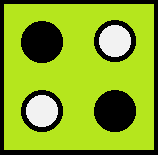
\includegraphics[scale=0.7]{img/_Cell1.png}
\caption{A Cell made of 4 Quantum Dots}
\label{img:cell}
\end{figure}

If we inject two electrons in this structure their reciprocal repulsion allow them to be only in two configurations, with the electrons disposed on one of the two diagonals. In order to let the system evolve electrons are allowed to move between dots inside a cell according to a clock signal but they can never exit the cell, the effect of the clock on the cells is explained in \ref{sec:clock}.
The configuration in picture \ref{img:cell} represents the logical bit 0 the opposite configuration is the bit 1. 
If we put two cells one beside the other we can see that the polarization of the first cells has an impact on the polarization of the other. This effect can be used to build complex logic circuits. Main blocks of QCA circuits are NOT and Majority Gate both shown in figure \ref{img:gates}.
\begin{figure}
\centering
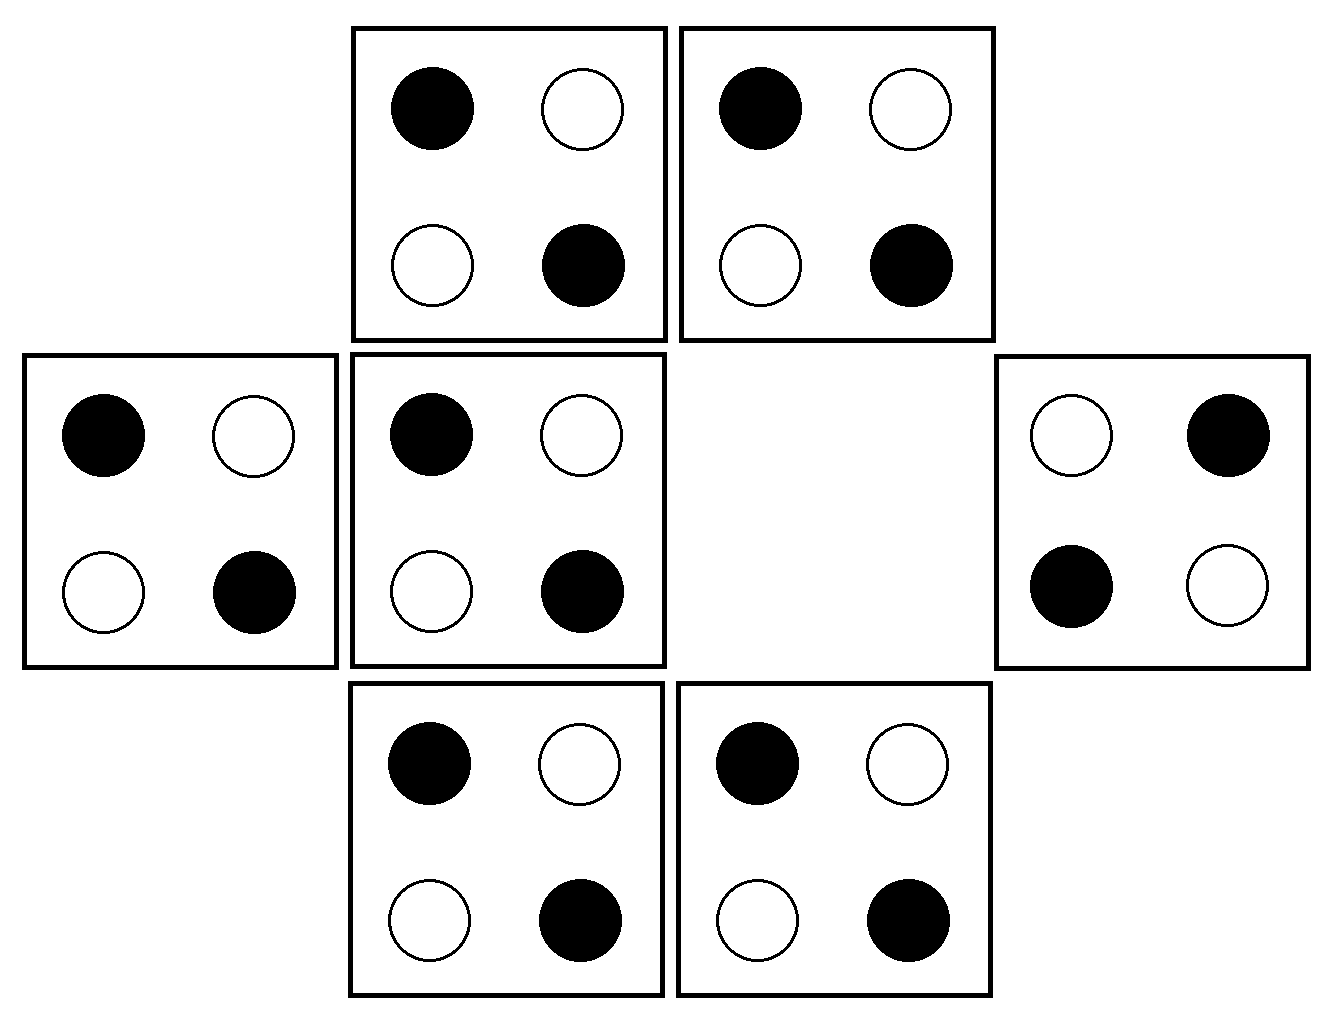
\includegraphics[scale=0.1]{img/not_normal.png}
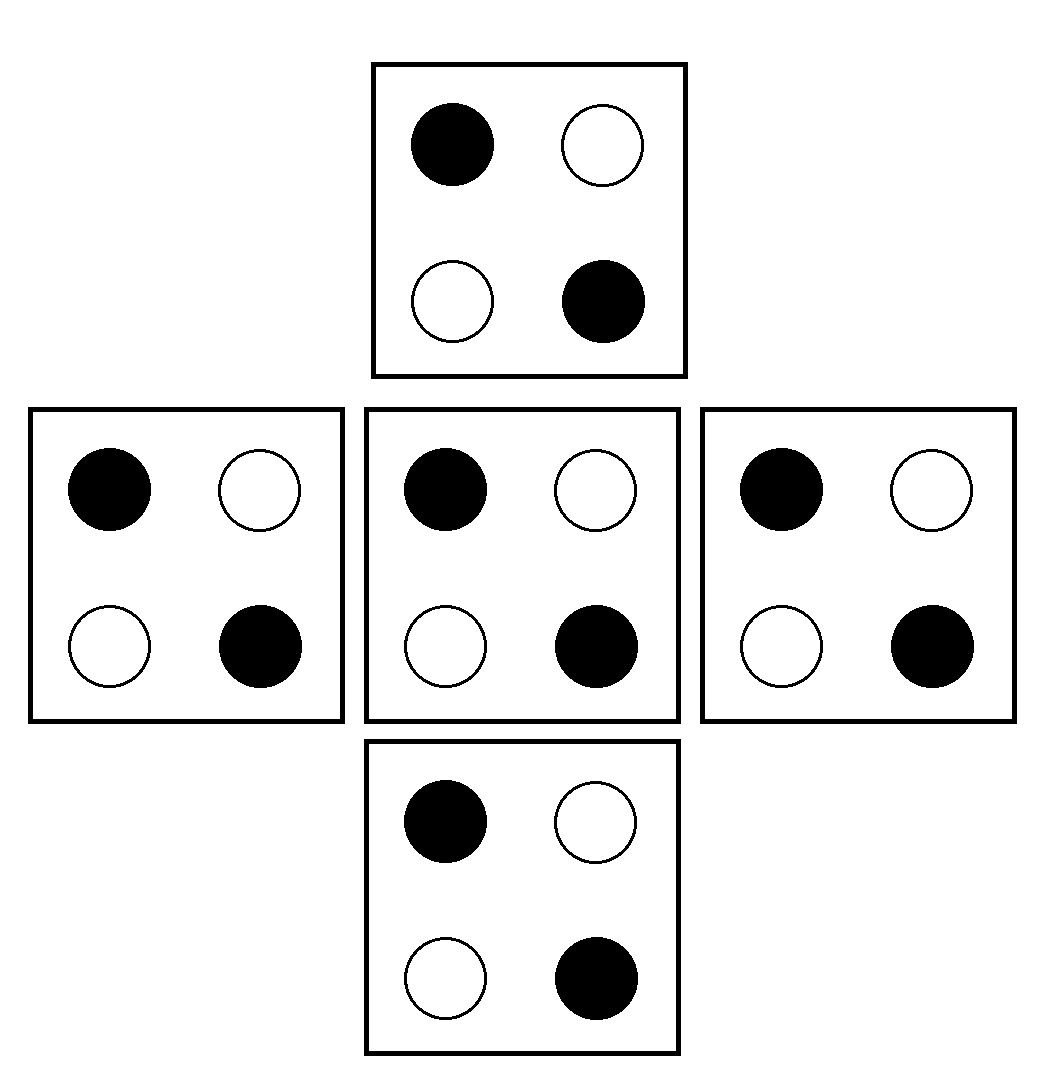
\includegraphics[scale=0.1]{img/majority.png}
\caption{NOT and majority gate}
\label{img:gates}
\end{figure}

\subsection{Clock}
\label{sec:clock}
A key issue in the design of circuits is the definition of clock areas. As said in \ref{sec:qca} in order to define the switching of cells polarization a clock signal is used. QCA uses 4 identical clock signals shifted of $\frac{\pi}{4}$. Each clock signal has 4 clock phases: switch, hold, release and relax. The wave form of the clock signal is shown in figure \ref{img:clock}. 

\begin{figure}
\centering
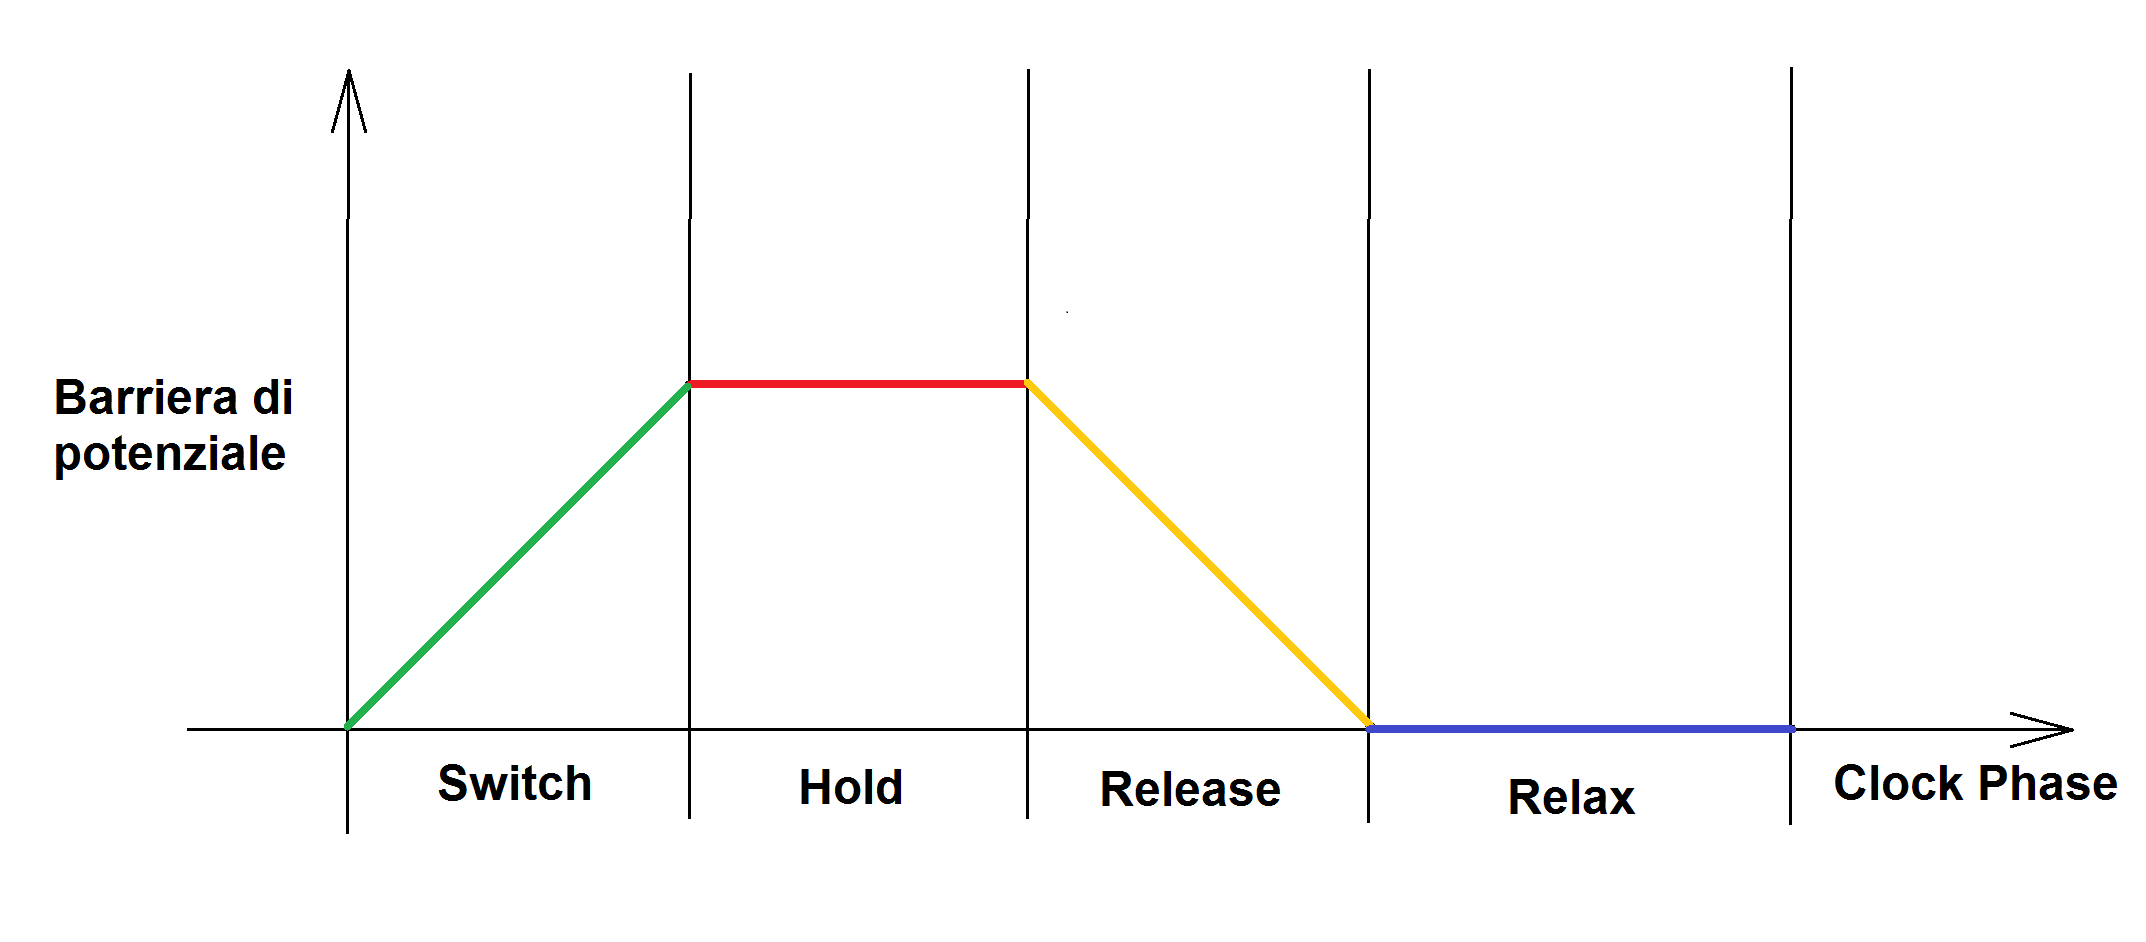
\includegraphics[scale=0.1]{img/clock.png}
\caption{NOT and majority gate}
\label{img:clock}
\end{figure}

During these phases potential barriers between dots inside the cell are raised or lowered in order to control the movement of electrons. In the relax phase barriers are low and electrons can freely move inside the cell, during the switch phase barriers are raised and the movement of electrons are limited. during the hold phase electrons are not allowed to move within dots. In the relax phase the barriers are lowered. \newline
In the design of circuits based on QCA the alternation of the four clock signals are used to control the flow of information. In figure \ref{img:ambiente} is shown a very simple circuit in which different cell colors correspond to different clock signals. At the beginning of the computation the input configurations are presented in the upper cells and at the end of the computation the output is read from the lower cell after a delay. The information flows from the input to the output according to the clock signals. The time that the information takes to go from the input to the output is the delay of the circuit. It can be easily seen from picture \ref{img:ambiente} that QCA is a pipeline technology so during the processing of a combination of inputs another combination can be presented to the input cells at each clock cycle. The total delay of the circuit is the number of cell signals switched from the inputs to the output divided by 4.

\section{QCADesigner}
QCADesigner is a tool made by the University of British Columbia to design and verify circuits in QCA technology. This tool offers two main feature. The first is to design with an intuitive graphical user interface a circuit, in the image \ref{img:ambiente} is showed the design GUI and a very simple circuit, the second is to simulate the behavior of the circuit. 

\begin{figure}
\centering
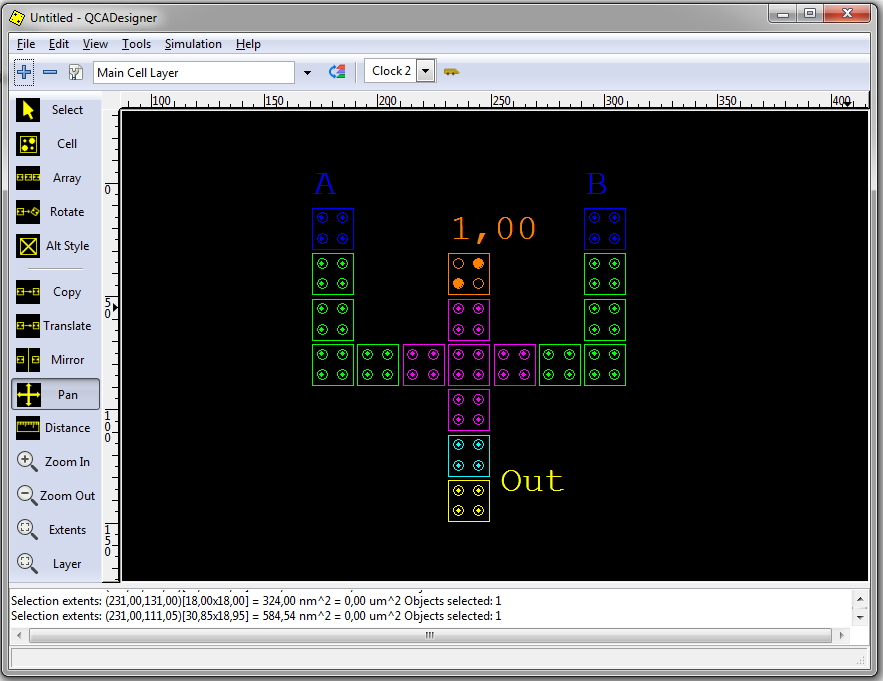
\includegraphics[scale=0.4]{img/QCADesigner.png}
\caption{QCADesigner GUI}
\label{img:ambiente}
\end{figure}
To verify the behavior of the system two simulation engines are offered. The bistable simulation and the coherence vector simulation. The goal of this project is to speedup the execution of the bistable simulation engine so we are going to briefly describe  how this simulation works. The coherence vector differs from the bistable simulation in the way the polarization of cells is calculated, it is much slower but gives more accurate result.

\subsection{Bistable Simulation}
Bistable simulation engine has been created in order to give designers a way to rapidly test their circuit during the design phase. For the simulation the cell is modelled as a two state system, for each cell the kink energy with respect to neighbor cells and the polarization is stored. The kink energy takes into account the cost of two neighboring cells having opposite polarizations. How the new polarization of each cell is calculated and details about the simulation algorithms are shown in\ref{sec:cpu_algorithm}. The modeling of the cells as a simple two state system is an approximations that this simulator engine does to be able verify the logical behavior of the system faster than the coherence vector engine by sacrificing the ability to describe well the dynamics of the circuit. 


\section{CUDA}
\label{sec:art_of_cuda}
   In recent times, Graphics Processing Units (GPUs) have been considered a potential source of computational
power for non-graphical applications, due to the ongoing evolution of their programming interfaces and their
appealing cost-performance figures of merit. Recent works had first attempted to adapt general purpose applications
to the graphic rendering APIs (OpenGL and DirectX), which up to two years ago represented the only interface to tap
into the GPU computational resources. Tesla is NVIDIA's first dedicated General Purpose GPU.
\newline
\subsection{NVIDIA Tesla Architecture}
   Modern GPUs include hundreds of processing elements. The NVIDIA Tesla GPU series provide a set
of independent multithreaded streaming multiprocessors. \figurename~\ref{fig:teslaarch} shows an overview of the NVIDIA
Tesla streaming processors array which is the part of the GPU architecture responsible for the general purpose computation.
Each streaming multiprocessor is composed by a set of eight streaming processors,two special functional units and a multithreaded
instruction issue unit (respectively indicated as SP, SFU and MT-Issue in \figurename~\ref{fig:teslaarch}).\newline
A SP is a fully pipelined single-issue processing core with two ALUs and a single floating point unit (FPU). 
SFUs are dedicated to the computation of transcendental functions and pixel/vertex manipulations.
The MT-Issue unit is in charge of mapping active threads on the available SPs.\newline
  A multiprocessor is able to concurrently execute groups of 32 threads called warps. Since each thread
in a warp has its own control flow, their execution paths may diverge due to the independent evaluation
of conditional statements. In this case, the warp serially executes each path. When the warp is executing
a given path, all threads that have not taken that path are disabled. On the other hand, in case the
control flows converge again, the warp may return to a single, parallel execution of all threads.\newline
 Each multiprocessor executes warps in a fashion much like the Single Instruction Multiple Data (SIMD)
paradigm, since every thread will be assigned to a different SP and every active thread will execute the
same instruction on different data.\newline
   The MT-Issue unit weaves threads into a number of warps and schedules an active warp for execution,
using a round-robin scheduling policy with aging for this purpose.\newline
   Streaming multiprocessors are in turn grouped in Texture Processor Clusters (TPC). Each TPC includes three streaming
multiprocessors in the Tesla architecture. The TPC also includes support for Texture processing, though these features are
seldom used for general purpose computing and will not be investigated in this description.\newline
   Finally, the NVIDIA GPU on-board memory hierarchy includes registers (private to each SP), on-chip memory and off-chip memory.
The on-chip memory is private to each multiprocessor, and is split into a very small instruction cache, a read-only data cache,
and 16 KB of addressable shared data, respectively indicated as I-cache, C-cache and Shared Memory in \figurename~\ref{fig:Tesla}.
This shared memory is organized in 16 banks that can be concurrently accessed, each bank having a single read/write port.\newline
  The GPU we used for our project is the NVIDIA Tesla c1060. 
 With the computational power of its 240 Streaming Processors (grouped into 30 TPCs) and the 102,4 GB/s max bandwidth of its 4096 MB
GDDR3 memory, it represents one of the most performing GPUs on the market.\newline

\begin{figure}[h]
    \centering
     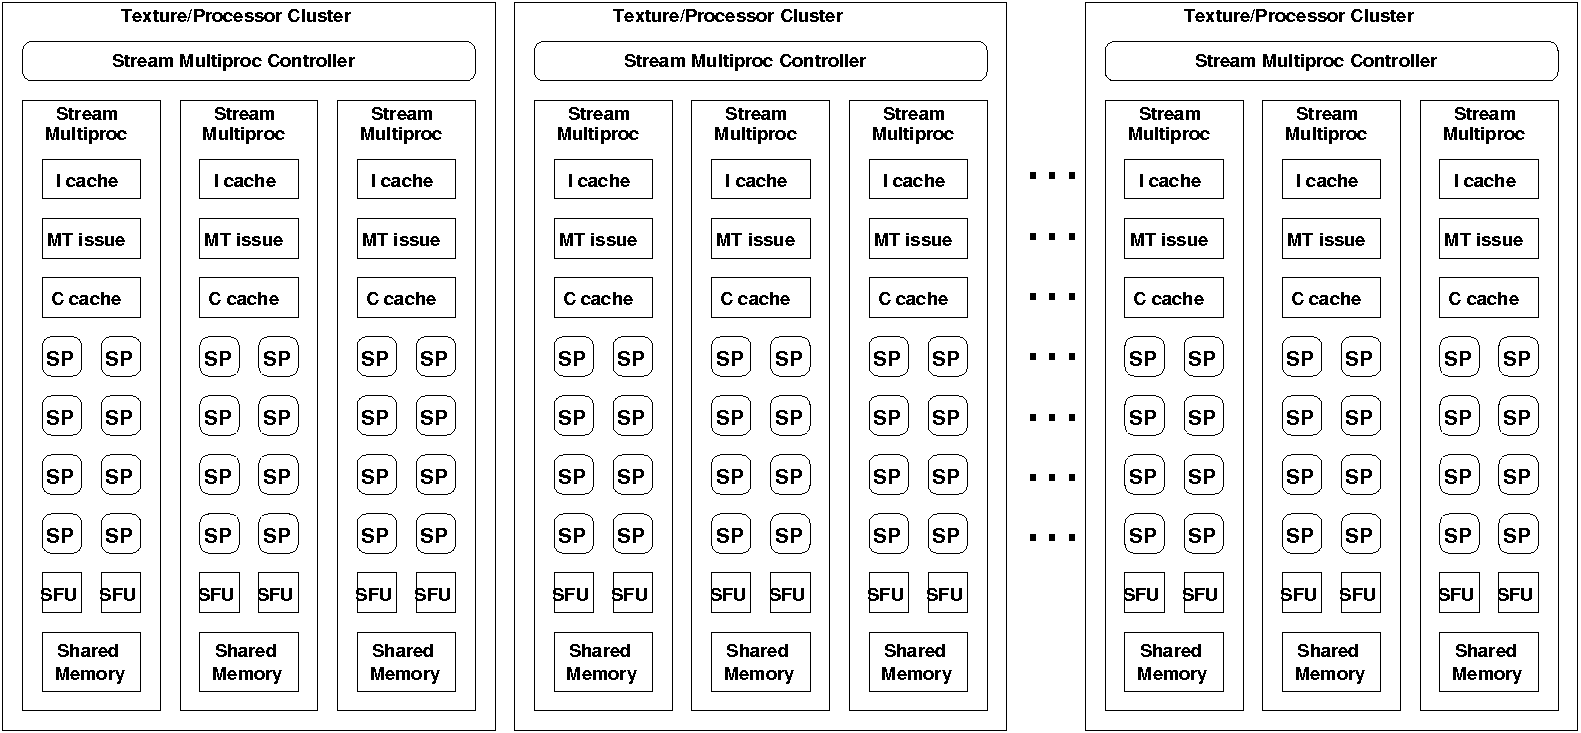
\includegraphics[width=1\textwidth]{./img/nvidiadetail}
\caption{Architectural detail of the Tesla Architecture}\label{fig:teslaarch}
    \end{figure}


\subsection{CUDA programming model}
   The Compute Unified Device Architecture (CUDA), proposed by NVIDIA for its GeForce (8 series and above), Quadro and Tesla
graphics processors, exposes a programming model that integrates host and GPU code in the same C/C++ source files.\newline
The main programming structure supporting parallelism is an explicitly parallel function invocation (kernel) which
is supposed to be executed by a user-specified number of threads.
Every kernel is explicitly invoked by host code and executed by the device, while the host-side code continues execution
 asynchronously after instantiating the kernel. The programmer is provided with a specific synchronizing function call
to wait for the completion of the active asynchronous kernel computation.\newline
   The CUDA programming model abstracts the actual parallelism implemented by the hardware architecture,
providing the concepts of block and thread to express concurrency in algorithms.
A block captures the notion of a group of concurrent threads. Blocks are required to execute independently, so that it has
to be possible to execute them in any order (in parallel or in sequence). Therefore, the synchronization primitives semantically
act only among threads belonging to the same block.
Intra-block communications among threads use the logical shared memory associated with that block.\newline
   Since the architecture does not provide support for the message-passing techniques, threads belonging
to different blocks must communicate through global memory. The global memory is entirely mapped to the off-chip memory.
The concurrent accesses to logical shared memory by threads executing within the same block are supported through an explicit
barrier synchronization primitive.\newline
   A kernel call-site must specify the number of blocks as well as the number of threads within each
block when executing the kernel code. The current CUDA programming model imposes a capping of 512 threads per block.\newline
   The mapping of threads to processors and of blocks to multiprocessors is mainly handled by hardware controller components.
Two or more blocks may share the same multiprocessor through mechanisms that allow fast context switching depending on 
the computational resources used by threads and on the constraints of the hardware architecture.
The number of concurrent blocks managed by a single multiprocessor is currently limited to 8.\newline
   In addition to the logical shared memory and the global memory, in the CUDA programming model each thread may access a constant memory.
 An access to this read-only memory space is faster than one to global memory, provided that there is sufficient access locality since
constant memory is implemented as a region of global memory fit with an on-chip cache.
Finally, another portion of the off-chip memory may be allocated as a local memory that is used as thread private resource.
Since the local memory access is slow, the shared memory also serves as an explicitly managed cache though it is up to the
programmer to warrant that the local data being saved in shared memory are not accessed by other
threads. Shared memory comes in limited amounts (threads within each block typically share 16 KB of memory) hence,
it is crucial for performance that each thread handle only small chunks of data.

\subsection{SIMT and SIMD}
   SIMT architecture is similar to single instruction, multiple-data (SIMD) design, which applies one instruction to multiple data lanes.\newline
 The difference is that SIMT applies one instruction to multiple independent threads in parallel, not just multiple data lanes.
A SIMD instruction controls a vector of multiple data lanes together and exposes the vector width to the software, whereas a SIMT instruction
controls the execution and branching behavior of one thread.\newline
   In contrast to SIMD vector architectures, SIMT enables programmers to write thread level parallel code for independent threads
as well as data-parallel code for coordinated threads.\newline
For program correctness, programmers can essentially ignore SIMT execution attributes such as warps; however, they can
achieve substantial performance improvements by writing code that seldom requires threads in a warp to diverge. In practice, this
is analogous to the role of cache lines in traditional codes: programmers can safely ignore cache line size when designing for
correctness but must consider it in the code structure when designing for peak performance.\newline 
SIMD vector architectures, on the other hand, require the software to manually coalesce loads into vectors and to manually manage
divergence.







